\SourceLeaf{414}%
\noindent [ist:]
\begin{equation}\tag{4}
\xi.\frac{\partial X}{\partial\theta}+\eta.\frac{\partial Y}{\partial\theta}+\zeta.\frac{\partial Z}{\partial\theta}=-mq
\end{equation}
\noindent [und]
\begin{equation}\tag{5}
\begin{aligned}
(YZ'-ZY')\frac{\partial X}{\partial\theta}+(ZX'-XZ')\frac{\partial Y}{\partial\theta}&\\
+(XY'-YX')\frac{\partial Z}{\partial\theta}&=\frac{\partial\partial m}{\partial r^2}.
\end{aligned}
\end{equation}
\indent Die Bedeutung der Gleichung (4) kann so versinnlicht werden. Es sind $dr$ und $md\theta$ zwei auf einander senkrechte Linearelemente auf der Fläche. Auf der Himmelskugel stellen $Q,Q',Q''$ resp. die Normalen in $P,P',P''$ vor. $QR'$ stellt vor die Verticalebene durch $PP'$, $QR''$ die Verticalebene durch $PP''$. Dann bedeutet:
\begin{center}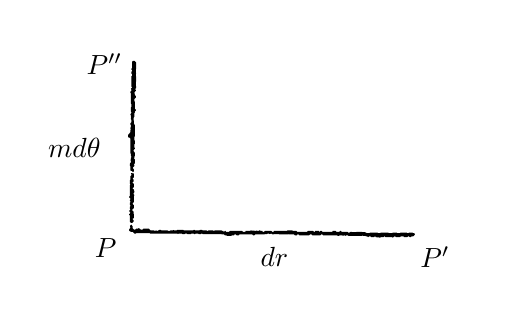
\begin{tikzpicture}[x=.00225in,y=-.00225in]
\path[use as bounding box] (0,0) rectangle (1015,567);
\path[fill=black,even odd rule] (226,450) -- (226,452) -- (228,454) -- (230,455) -- (234,455) -- (238,459) -- (241,459) -- (242,458) -- (272,458) -- (273,459) -- (334,459) -- (335,460) -- (337,459) -- (344,459) -- (345,460) -- (350,460) -- (351,459) -- (355,459) -- (356,460) -- (364,460) -- (365,459) -- (370,459) -- (371,460) -- (373,460) -- (374,459) -- (380,459) -- (381,460) -- (386,460) -- (387,459) -- (389,459) -- (390,460) -- (432,460) -- (433,461) -- (438,461) -- (440,463) -- (443,463) -- (444,464) -- (454,464) -- (455,463) -- (460,463) -- (461,461) -- (464,461) -- (466,463) -- (470,463) -- (472,461) -- (501,461) -- (503,463) -- (505,463) -- (507,461) -- (528,461) -- (529,460) -- (534,460) -- (535,459) -- (538,459) -- (539,460) -- (543,459) -- (546,461) -- (548,461) -- (549,460) -- (560,460) -- (561,461) -- (580,461) -- (582,460) -- (583,461) -- (594,461) -- (596,463) -- (600,463) -- (601,461) -- (604,461) -- (606,463) -- (627,463) -- (629,461) -- (633,461) -- (635,463) -- (652,463) -- (654,461) -- (657,461) -- (659,463) -- (690,463) -- (691,464) -- (694,464) -- (695,463) -- (702,463) -- (703,464) -- (705,463) -- (707,463) -- (708,464) -- (710,463) -- (714,463) -- (715,464) -- (745,464) -- (747,463) -- (748,464) -- (753,464) -- (754,465) -- (757,465) -- (759,467) -- (761,465) -- (764,465) -- (766,467) -- (772,467) -- (774,465) -- (775,465) -- (776,467) -- (786,468) -- (787,467) -- (793,467) -- (795,465) -- (796,465) -- (798,467) -- (812,467) -- (814,468) -- (818,465) -- (819,465) -- (821,467) -- (830,467) -- (832,465) -- (838,465) -- (839,467) -- (846,467) -- (848,465) -- (850,465) -- (852,467) -- (854,467) -- (856,465) -- (859,465) -- (861,464) -- (863,461) -- (863,460) -- (861,458) -- (859,458) -- (858,457) -- (850,457) -- (849,458) -- (846,458) -- (845,457) -- (831,457) -- (830,458) -- (824,458) -- (823,457) -- (814,457) -- (813,458) -- (805,458) -- (804,457) -- (787,457) -- (786,458) -- (781,458) -- (780,457) -- (763,457) -- (762,458) -- (756,458) -- (752,456) -- (746,456) -- (745,455) -- (733,455) -- (732,456) -- (723,456) -- (722,455) -- (720,455) -- (717,457) -- (715,457) -- (713,455) -- (700,455) -- (698,453) -- (697,453) -- (695,455) -- (688,455) -- (686,453) -- (680,453) -- (679,455) -- (657,455) -- (655,453) -- (653,453) -- (651,455) -- (650,455) -- (649,453) -- (641,453) -- (640,455) -- (638,455) -- (636,453) -- (625,453) -- (623,455) -- (601,455) -- (599,453) -- (591,453) -- (590,452) -- (579,452) -- (578,453) -- (549,453) -- (548,455) -- (545,455) -- (543,453) -- (529,453) -- (527,455) -- (524,455) -- (523,453) -- (519,453) -- (518,452) -- (516,452) -- (515,453) -- (512,453) -- (511,452) -- (509,453) -- (497,452) -- (496,453) -- (486,453) -- (485,455) -- (480,455) -- (478,453) -- (451,453) -- (449,455) -- (442,455) -- (441,453) -- (440,453) -- (438,455) -- (437,455) -- (436,453) -- (433,453) -- (432,452) -- (417,452) -- (416,453) -- (414,453) -- (413,452) -- (403,452) -- (402,453) -- (400,453) -- (399,452) -- (390,452) -- (389,451) -- (384,451) -- (383,452) -- (373,452) -- (372,451) -- (370,451) -- (369,452) -- (348,452) -- (347,451) -- (333,451) -- (332,452) -- (327,452) -- (325,451) -- (324,452) -- (318,452) -- (317,453) -- (313,453) -- (312,452) -- (298,452) -- (297,451) -- (293,451) -- (290,453) -- (288,453) -- (287,452) -- (283,453) -- (282,452) -- (274,452) -- (271,449) -- (271,448) -- (258,448) -- (256,450) -- (252,450) -- (250,448) -- (247,447) -- (246,448) -- (242,448) -- (240,450) -- (237,450) -- (234,447) -- (234,443) -- (231,439) -- (228,442) -- (229,446) -- cycle (231,324) -- (230,325) -- (231,326) -- (231,329) -- (229,331) -- (229,339) -- (228,340) -- (228,348) -- (229,349) -- (228,351) -- (228,375) -- (226,377) -- (226,378) -- (229,381) -- (229,383) -- (228,384) -- (228,386) -- (229,387) -- (229,389) -- (228,390) -- (228,395) -- (229,396) -- (229,398) -- (228,399) -- (228,404) -- (229,406) -- (227,408) -- (226,408) -- (229,413) -- (226,416) -- (226,417) -- (228,419) -- (228,433) -- (230,435) -- (233,435) -- (236,432) -- (236,429) -- (234,427) -- (234,426) -- (237,424) -- (237,416) -- (236,415) -- (236,410) -- (233,407) -- (233,406) -- (237,402) -- (237,396) -- (234,393) -- (234,392) -- (237,388) -- (237,375) -- (238,373) -- (236,371) -- (236,369) -- (238,367) -- (238,364) -- (237,363) -- (237,361) -- (234,359) -- (234,358) -- (237,355) -- (237,349) -- (234,346) -- (234,344) -- (236,343) -- (236,339) -- (234,337) -- (234,336) -- (237,333) -- (237,326) -- (236,325) -- cycle (238,74) -- (235,74) -- (233,76) -- (233,90) -- (231,92) -- (231,93) -- (233,95) -- (233,97) -- (231,98) -- (231,102) -- (233,104) -- (233,107) -- (231,108) -- (231,131) -- (233,133) -- (230,136) -- (231,138) -- (231,141) -- (229,143) -- (229,145) -- (230,146) -- (230,169) -- (231,170) -- (231,177) -- (230,178) -- (230,187) -- (231,188) -- (231,190) -- (229,194) -- (230,195) -- (230,198) -- (231,199) -- (230,201) -- (230,204) -- (231,205) -- (231,211) -- (229,213) -- (229,216) -- (230,217) -- (230,222) -- (229,223) -- (229,225) -- (230,226) -- (229,228) -- (229,233) -- (224,239) -- (224,243) -- (225,245) -- (227,245) -- (229,247) -- (229,280) -- (230,281) -- (230,286) -- (231,287) -- (231,289) -- (230,290) -- (230,294) -- (229,295) -- (230,297) -- (230,300) -- (228,303) -- (228,308) -- (229,309) -- (229,318) -- (230,319) -- (232,319) -- (234,321) -- (234,322) -- (235,322) -- (237,320) -- (237,317) -- (234,312) -- (238,308) -- (237,304) -- (239,302) -- (239,294) -- (237,292) -- (238,290) -- (238,287) -- (239,286) -- (239,279) -- (236,275) -- (236,273) -- (239,270) -- (239,268) -- (238,267) -- (238,260) -- (239,259) -- (239,252) -- (238,251) -- (238,243) -- (239,242) -- (239,218) -- (237,214) -- (236,201) -- (238,198) -- (238,190) -- (239,189) -- (239,187) -- (241,185) -- (241,183) -- (239,181) -- (239,165) -- (238,164) -- (238,159) -- (241,156) -- (241,152) -- (239,151) -- (238,144) -- (241,141) -- (241,139) -- (239,137) -- (242,134) -- (242,131) -- (241,130) -- (241,121) -- (242,120) -- (242,109) -- (241,108) -- (241,103) -- (242,102) -- (241,100) -- (241,93) -- (242,92) -- (242,78) -- cycle;
\node[inner sep=0pt,font=\normalsize] at (171,82) {$P''$};
\node[inner sep=0pt,font=\normalsize] at (104,268) {$md\theta$};
\node[inner sep=0pt,font=\normalsize] at (174,492) {$P$};
\node[inner sep=0pt,font=\normalsize] at (550,512) {$dr$};
\node[inner sep=0pt,font=\normalsize] at (908,512) {$P'$};
\end{tikzpicture}
\end{center}
\noindent\hspace*{1.2em}Gleichung (4), dass
\[
\frac{Q''R''}{PP''}=\frac{Q'R'}{PP'},
\]
\begin{center}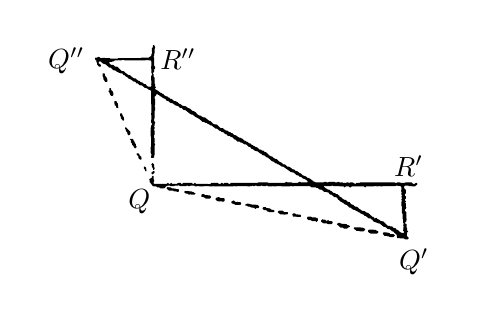
\begin{tikzpicture}[x=.00225in,y=-.00225in]
\path[use as bounding box] (0,0) rectangle (959,602);
\path[fill=black,even odd rule] (792,458) -- (792,460) -- (795,464) -- (801,464) -- (802,465) -- (805,465) -- (807,467) -- (815,467) -- (819,463) -- (815,460) -- (808,460) -- (807,458) -- (805,458) -- (804,457) -- (794,456) -- cycle (759,452) -- (759,455) -- (761,457) -- (765,459) -- (779,459) -- (782,456) -- (782,455) -- (780,453) -- (778,453) -- (776,451) -- (772,451) -- (771,450) -- (761,450) -- cycle (727,446) -- (727,449) -- (730,450) -- (733,453) -- (739,453) -- (740,454) -- (749,454) -- (752,451) -- (752,449) -- (750,447) -- (748,447) -- (747,446) -- (743,446) -- (742,445) -- (728,445) -- cycle (689,438) -- (698,446) -- (703,446) -- (705,448) -- (712,448) -- (714,446) -- (718,444) -- (718,442) -- (717,442) -- (715,440) -- (713,440) -- (711,438) -- (699,437) -- (695,435) -- (693,435) -- cycle (654,430) -- (654,432) -- (656,434) -- (660,436) -- (667,436) -- (669,438) -- (677,438) -- (680,435) -- (680,433) -- (677,431) -- (672,431) -- (670,429) -- (666,431) -- (663,428) -- (659,428) -- (657,427) -- cycle (623,423) -- (623,426) -- (626,429) -- (631,429) -- (634,431) -- (642,431) -- (643,433) -- (644,433) -- (647,430) -- (647,426) -- (645,424) -- (643,424) -- (642,423) -- (634,423) -- (631,421) -- (625,421) -- cycle (590,416) -- (591,420) -- (592,421) -- (599,421) -- (600,422) -- (608,422) -- (609,421) -- (609,418) -- (608,417) -- (598,416) -- (596,414) -- (592,414) -- cycle (558,410) -- (558,412) -- (563,416) -- (570,416) -- (571,417) -- (574,417) -- (575,416) -- (579,416) -- (580,415) -- (580,412) -- (579,411) -- (572,411) -- (568,408) -- (560,408) -- cycle (524,402) -- (524,404) -- (526,406) -- (528,407) -- (532,407) -- (535,410) -- (537,410) -- (538,411) -- (549,411) -- (550,410) -- (550,408) -- (548,406) -- (544,406) -- (540,403) -- (532,402) -- (531,400) -- (526,400) -- cycle (485,395) -- (485,396) -- (489,397) -- (491,399) -- (495,399) -- (499,401) -- (503,401) -- (504,402) -- (506,402) -- (507,404) -- (508,404) -- (510,402) -- (514,402) -- (516,400) -- (516,398) -- (512,395) -- (497,394) -- (496,393) -- (493,393) -- (492,392) -- (487,393) -- cycle (454,388) -- (454,390) -- (456,392) -- (458,392) -- (460,394) -- (462,394) -- (463,395) -- (474,395) -- (476,393) -- (476,391) -- (474,389) -- (469,389) -- (468,388) -- (464,389) -- (459,385) -- cycle (419,381) -- (419,384) -- (424,387) -- (433,387) -- (434,388) -- (437,388) -- (439,386) -- (439,382) -- (438,380) -- (431,380) -- (427,378) -- (424,378) -- (423,379) -- (421,379) -- cycle (387,373) -- (387,376) -- (388,377) -- (393,378) -- (397,381) -- (406,381) -- (409,378) -- (409,377) -- (406,374) -- (395,373) -- (393,371) -- (389,371) -- cycle (349,366) -- (349,367) -- (351,368) -- (352,370) -- (357,370) -- (359,372) -- (361,372) -- (362,371) -- (364,372) -- (372,372) -- (374,370) -- (374,369) -- (371,368) -- (369,366) -- (366,366) -- (365,365) -- (351,364) -- cycle (310,357) -- (310,359) -- (315,363) -- (324,363) -- (326,365) -- (332,365) -- (333,366) -- (336,366) -- (337,364) -- (337,361) -- (336,360) -- (331,360) -- (330,359) -- (327,359) -- (326,358) -- (321,358) -- (319,356) -- (314,356) -- (313,355) -- (312,355) -- cycle (282,320) -- (280,320) -- (276,323) -- (276,325) -- (278,327) -- (279,327) -- (283,323) -- (283,321) -- cycle (259,310) -- (259,314) -- (261,316) -- (262,320) -- (265,320) -- (264,312) -- (262,310) -- cycle (278,302) -- (276,304) -- (276,306) -- (277,307) -- (277,311) -- (279,313) -- (280,317) -- (281,317) -- (283,315) -- (283,312) -- (282,311) -- (282,306) -- (281,304) -- (279,302) -- cycle (244,280) -- (243,281) -- (243,283) -- (247,287) -- (247,291) -- (250,294) -- (253,294) -- (254,293) -- (253,287) -- (252,287) -- (249,284) -- (249,282) -- (247,280) -- cycle (228,248) -- (228,249) -- (230,251) -- (230,255) -- (233,259) -- (233,261) -- (236,264) -- (236,266) -- (239,269) -- (240,269) -- (243,266) -- (243,265) -- (241,263) -- (241,260) -- (238,255) -- (238,253) -- (236,252) -- (236,250) -- (234,248) -- cycle (217,222) -- (217,225) -- (219,228) -- (219,230) -- (222,234) -- (222,237) -- (225,240) -- (226,240) -- (229,237) -- (229,233) -- (228,231) -- (220,223) -- (220,222) -- cycle (207,191) -- (206,192) -- (206,197) -- (208,199) -- (208,202) -- (212,207) -- (214,207) -- (215,206) -- (214,199) -- (212,197) -- (210,191) -- cycle (194,164) -- (193,165) -- (194,173) -- (195,173) -- (197,175) -- (197,177) -- (199,179) -- (201,179) -- (202,178) -- (201,169) -- (199,167) -- (199,165) -- (197,164) -- cycle (183,135) -- (182,136) -- (182,140) -- (180,141) -- (180,142) -- (182,144) -- (184,150) -- (186,152) -- (189,152) -- (191,150) -- (191,145) -- (190,144) -- (190,142) -- (189,142) -- (186,139) -- (186,136) -- (185,135) -- cycle (168,102) -- (167,103) -- (167,108) -- (169,112) -- (169,115) -- (173,121) -- (176,121) -- (178,119) -- (177,113) -- (172,106) -- (172,103) -- (171,102) -- cycle (150,68) -- (151,72) -- (153,73) -- (153,76) -- (155,79) -- (155,82) -- (159,87) -- (162,87) -- (163,86) -- (163,83) -- (158,79) -- (158,77) -- (160,75) -- (162,75) -- (168,80) -- (174,82) -- (182,89) -- (185,89) -- (190,94) -- (192,95) -- (195,95) -- (200,99) -- (202,99) -- (204,101) -- (206,101) -- (207,102) -- (211,102) -- (214,106) -- (216,106) -- (219,109) -- (222,110) -- (226,114) -- (231,116) -- (236,120) -- (239,120) -- (242,123) -- (242,124) -- (245,124) -- (249,128) -- (255,129) -- (261,134) -- (263,134) -- (267,136) -- (269,138) -- (273,139) -- (275,141) -- (275,170) -- (276,171) -- (276,190) -- (275,191) -- (275,194) -- (276,195) -- (276,205) -- (275,206) -- (275,211) -- (277,213) -- (277,216) -- (275,219) -- (275,222) -- (274,223) -- (274,225) -- (275,226) -- (274,228) -- (274,242) -- (275,243) -- (275,265) -- (274,266) -- (274,271) -- (275,273) -- (274,274) -- (274,279) -- (276,282) -- (276,285) -- (275,286) -- (275,289) -- (276,290) -- (280,290) -- (282,289) -- (282,285) -- (283,284) -- (283,262) -- (284,261) -- (284,259) -- (282,257) -- (283,255) -- (283,247) -- (282,246) -- (282,239) -- (283,238) -- (283,230) -- (282,229) -- (282,226) -- (283,225) -- (283,222) -- (282,221) -- (282,219) -- (283,218) -- (283,214) -- (284,213) -- (284,211) -- (282,208) -- (282,203) -- (283,202) -- (283,185) -- (284,184) -- (284,177) -- (283,176) -- (283,174) -- (284,173) -- (284,159) -- (283,158) -- (283,154) -- (286,151) -- (286,150) -- (288,148) -- (289,148) -- (291,150) -- (293,150) -- (295,153) -- (297,153) -- (302,157) -- (307,159) -- (310,163) -- (314,164) -- (317,167) -- (324,169) -- (329,173) -- (336,175) -- (340,179) -- (343,179) -- (347,183) -- (352,184) -- (362,192) -- (366,194) -- (368,194) -- (374,199) -- (376,199) -- (377,201) -- (379,201) -- (381,203) -- (382,203) -- (390,210) -- (393,210) -- (396,212) -- (399,212) -- (402,215) -- (404,215) -- (407,218) -- (410,218) -- (419,225) -- (422,225) -- (428,230) -- (430,230) -- (432,232) -- (436,233) -- (440,237) -- (444,238) -- (446,241) -- (450,241) -- (453,244) -- (456,244) -- (461,249) -- (464,250) -- (468,254) -- (473,254) -- (475,256) -- (477,256) -- (483,260) -- (486,260) -- (488,261) -- (493,266) -- (496,266) -- (499,270) -- (501,270) -- (506,274) -- (513,276) -- (519,281) -- (521,281) -- (523,284) -- (528,285) -- (531,288) -- (536,290) -- (545,298) -- (549,299) -- (552,302) -- (556,303) -- (558,305) -- (560,305) -- (567,310) -- (570,310) -- (587,322) -- (593,323) -- (600,329) -- (603,329) -- (605,331) -- (605,332) -- (607,332) -- (611,334) -- (613,336) -- (619,338) -- (624,342) -- (624,344) -- (623,345) -- (609,345) -- (608,344) -- (605,344) -- (602,346) -- (589,346) -- (588,345) -- (579,345) -- (578,344) -- (576,344) -- (573,346) -- (536,346) -- (535,345) -- (514,345) -- (513,346) -- (453,346) -- (451,348) -- (448,348) -- (446,346) -- (439,346) -- (437,348) -- (436,348) -- (434,346) -- (432,346) -- (430,348) -- (426,348) -- (424,346) -- (410,346) -- (408,348) -- (406,348) -- (405,349) -- (403,349) -- (402,348) -- (375,348) -- (373,346) -- (372,346) -- (371,348) -- (368,348) -- (366,346) -- (347,346) -- (345,348) -- (342,348) -- (341,346) -- (335,346) -- (333,348) -- (322,348) -- (320,346) -- (319,346) -- (318,348) -- (315,348) -- (313,346) -- (312,346) -- (310,348) -- (282,348) -- (281,347) -- (281,344) -- (282,343) -- (282,339) -- (281,338) -- (281,331) -- (279,330) -- (277,332) -- (277,334) -- (275,336) -- (273,336) -- (271,338) -- (272,340) -- (272,344) -- (279,353) -- (281,354) -- (287,354) -- (289,356) -- (293,356) -- (296,358) -- (304,358) -- (306,357) -- (309,353) -- (311,353) -- (312,352) -- (317,352) -- (318,353) -- (327,353) -- (328,352) -- (335,352) -- (336,351) -- (340,353) -- (354,353) -- (355,352) -- (357,352) -- (358,353) -- (362,353) -- (363,352) -- (371,352) -- (374,354) -- (376,354) -- (377,353) -- (382,353) -- (383,354) -- (392,354) -- (393,353) -- (404,353) -- (405,354) -- (413,354) -- (414,353) -- (416,354) -- (426,354) -- (427,353) -- (429,354) -- (458,354) -- (459,353) -- (463,353) -- (464,354) -- (466,354) -- (467,353) -- (489,353) -- (490,354) -- (495,354) -- (496,353) -- (500,353) -- (501,352) -- (503,353) -- (506,353) -- (507,352) -- (510,352) -- (511,353) -- (519,353) -- (520,352) -- (523,352) -- (524,353) -- (531,353) -- (532,352) -- (534,352) -- (537,354) -- (545,354) -- (546,353) -- (548,353) -- (549,354) -- (554,354) -- (555,353) -- (565,353) -- (566,354) -- (584,354) -- (585,353) -- (589,353) -- (590,354) -- (592,354) -- (593,353) -- (629,353) -- (633,356) -- (643,356) -- (644,357) -- (646,357) -- (651,361) -- (655,361) -- (661,366) -- (666,366) -- (667,367) -- (670,367) -- (674,372) -- (677,372) -- (684,378) -- (688,378) -- (691,381) -- (691,382) -- (698,388) -- (704,391) -- (707,394) -- (711,395) -- (717,401) -- (720,401) -- (723,404) -- (727,406) -- (729,406) -- (733,409) -- (735,409) -- (737,411) -- (740,412) -- (742,414) -- (746,416) -- (748,416) -- (750,418) -- (750,419) -- (754,420) -- (760,425) -- (764,425) -- (767,428) -- (768,428) -- (772,433) -- (774,433) -- (781,436) -- (784,436) -- (794,444) -- (797,444) -- (803,449) -- (807,449) -- (813,454) -- (816,455) -- (817,457) -- (822,461) -- (823,463) -- (823,468) -- (824,469) -- (839,470) -- (841,472) -- (847,472) -- (849,470) -- (849,468) -- (845,464) -- (846,456) -- (848,455) -- (848,454) -- (846,452) -- (846,447) -- (845,446) -- (845,438) -- (841,436) -- (841,435) -- (844,432) -- (845,426) -- (844,425) -- (844,411) -- (841,408) -- (841,406) -- (843,404) -- (843,402) -- (844,401) -- (843,399) -- (843,392) -- (841,390) -- (843,388) -- (843,387) -- (841,385) -- (841,383) -- (843,381) -- (843,376) -- (841,374) -- (841,371) -- (843,369) -- (843,362) -- (840,359) -- (839,357) -- (839,354) -- (841,352) -- (849,352) -- (850,353) -- (863,354) -- (869,349) -- (869,348) -- (867,346) -- (865,346) -- (863,348) -- (859,348) -- (856,345) -- (842,345) -- (841,346) -- (831,346) -- (830,345) -- (824,345) -- (823,346) -- (819,346) -- (818,345) -- (741,345) -- (740,346) -- (733,346) -- (731,348) -- (729,348) -- (727,346) -- (725,346) -- (724,345) -- (719,345) -- (718,346) -- (716,346) -- (715,345) -- (711,345) -- (710,346) -- (703,346) -- (702,345) -- (698,345) -- (697,346) -- (694,344) -- (691,344) -- (690,345) -- (685,345) -- (684,344) -- (671,344) -- (670,345) -- (667,345) -- (666,344) -- (661,344) -- (660,345) -- (642,345) -- (639,343) -- (637,343) -- (636,341) -- (635,341) -- (630,337) -- (626,335) -- (624,335) -- (621,332) -- (613,329) -- (609,325) -- (606,324) -- (601,320) -- (597,319) -- (594,316) -- (591,316) -- (586,312) -- (582,310) -- (579,310) -- (574,305) -- (570,305) -- (568,303) -- (568,302) -- (560,298) -- (555,293) -- (553,293) -- (549,291) -- (545,287) -- (542,287) -- (540,285) -- (539,285) -- (532,278) -- (528,277) -- (526,275) -- (526,274) -- (522,274) -- (520,272) -- (517,272) -- (513,268) -- (509,266) -- (507,266) -- (506,264) -- (504,264) -- (502,262) -- (499,261) -- (496,258) -- (494,258) -- (489,254) -- (487,254) -- (485,252) -- (483,252) -- (481,250) -- (481,249) -- (480,249) -- (478,247) -- (476,247) -- (474,245) -- (471,245) -- (464,240) -- (460,239) -- (456,235) -- (454,235) -- (452,233) -- (449,233) -- (446,230) -- (441,229) -- (435,224) -- (431,224) -- (429,223) -- (422,216) -- (414,215) -- (407,208) -- (405,208) -- (395,200) -- (392,200) -- (388,198) -- (386,196) -- (383,196) -- (379,194) -- (374,188) -- (373,188) -- (371,186) -- (368,186) -- (361,180) -- (357,179) -- (355,177) -- (351,175) -- (345,174) -- (340,170) -- (338,170) -- (334,166) -- (330,164) -- (327,164) -- (321,159) -- (318,159) -- (316,156) -- (314,156) -- (311,153) -- (309,153) -- (305,151) -- (303,149) -- (303,148) -- (301,148) -- (299,146) -- (296,145) -- (291,141) -- (284,137) -- (284,135) -- (286,133) -- (284,131) -- (284,126) -- (283,125) -- (283,112) -- (281,109) -- (281,104) -- (279,102) -- (279,101) -- (282,98) -- (282,93) -- (284,91) -- (284,87) -- (282,85) -- (282,67) -- (281,66) -- (281,64) -- (282,63) -- (282,58) -- (283,57) -- (283,47) -- (284,46) -- (284,43) -- (282,39) -- (280,39) -- (279,40) -- (279,44) -- (277,46) -- (277,54) -- (278,56) -- (276,59) -- (276,61) -- (275,63) -- (273,65) -- (271,65) -- (270,67) -- (253,67) -- (252,68) -- (202,68) -- (201,69) -- (184,69) -- (183,68) -- (172,68) -- (171,67) -- (163,68) -- (159,65) -- (157,65) -- (155,67) -- (151,67) -- cycle (660,354) -- (662,352) -- (663,353) -- (677,353) -- (678,352) -- (680,352) -- (681,353) -- (695,353) -- (696,354) -- (704,354) -- (706,356) -- (707,356) -- (709,354) -- (716,354) -- (718,356) -- (720,356) -- (722,354) -- (750,354) -- (752,356) -- (753,356) -- (754,354) -- (771,354) -- (772,353) -- (778,353) -- (779,354) -- (781,354) -- (782,353) -- (785,353) -- (786,354) -- (791,354) -- (792,353) -- (820,353) -- (821,352) -- (831,353) -- (833,355) -- (833,362) -- (832,364) -- (834,367) -- (833,369) -- (833,372) -- (834,373) -- (834,376) -- (833,377) -- (834,379) -- (834,382) -- (833,383) -- (834,385) -- (834,387) -- (833,388) -- (833,397) -- (834,398) -- (834,413) -- (836,415) -- (836,426) -- (837,427) -- (837,435) -- (838,436) -- (838,439) -- (837,440) -- (838,442) -- (837,453) -- (839,455) -- (839,456) -- (837,458) -- (833,457) -- (829,455) -- (825,451) -- (823,451) -- (820,447) -- (816,447) -- (812,443) -- (808,443) -- (807,442) -- (804,442) -- (802,441) -- (793,432) -- (787,431) -- (785,429) -- (779,426) -- (778,424) -- (776,424) -- (774,426) -- (771,422) -- (769,422) -- (759,413) -- (755,412) -- (751,409) -- (745,408) -- (743,406) -- (739,404) -- (735,400) -- (733,399) -- (730,399) -- (726,395) -- (722,394) -- (718,390) -- (718,389) -- (713,388) -- (709,384) -- (707,384) -- (703,382) -- (699,378) -- (697,378) -- (695,376) -- (695,375) -- (691,372) -- (691,371) -- (688,371) -- (685,369) -- (681,368) -- (677,364) -- (675,364) -- (672,361) -- (669,361) -- (667,359) -- (664,358) -- cycle (182,77) -- (183,76) -- (188,76) -- (189,75) -- (192,75) -- (194,73) -- (202,73) -- (203,72) -- (205,73) -- (209,73) -- (210,72) -- (215,72) -- (216,73) -- (262,73) -- (263,72) -- (274,73) -- (276,76) -- (276,86) -- (275,87) -- (275,91) -- (276,92) -- (276,101) -- (277,102) -- (277,105) -- (275,109) -- (275,117) -- (276,118) -- (276,124) -- (275,126) -- (276,127) -- (276,130) -- (274,132) -- (267,131) -- (263,126) -- (260,126) -- (255,122) -- (251,121) -- (250,119) -- (246,118) -- (240,113) -- (237,113) -- (235,112) -- (228,106) -- (225,106) -- (223,104) -- (222,104) -- (214,97) -- (210,97) -- (201,88) -- (199,87) -- (195,87) -- (191,83) -- (186,83) -- (182,79) -- cycle;
\node[inner sep=0pt,font=\normalsize] at (86,74) {$Q''$};
\node[inner sep=0pt,font=\normalsize] at (335,71) {$R''$};
\node[inner sep=0pt,font=\normalsize] at (249,388) {$Q$};
\node[inner sep=0pt,font=\normalsize] at (849,308) {$R'$};
\node[inner sep=0pt,font=\normalsize] at (861,523) {$Q'$};
\end{tikzpicture}
\end{center}
\noindent\hspace*{1.2em}Gleichung (5), dass die Fläche
\[
2QQ'Q''=\frac{\partial\partial m}{m\partial r^2}PP'.PP''.
\]
\par\Needspace{9\baselineskip}\begin{center}\textbf{BEMERKUNG.}\end{center}
\noindent\hspace*{1.2em}Die vorstehende Notiz findet sich in einem Handbuche. Sie stammt vermuthlich aus dem Jahre 1825 und enthält Ergebnisse der Forschungen, die \textsc{Gauss} in den nachfolgend abgedruckten \textit{Neuen allgemeinen Untersuchungen über die krummen Flächen} ausführlich darzustellen begonnen hat.
\begin{flushright}\textsc{Stäckel}.\end{flushright}
